\section{Method}

%\begin{figure*}[th!]
%  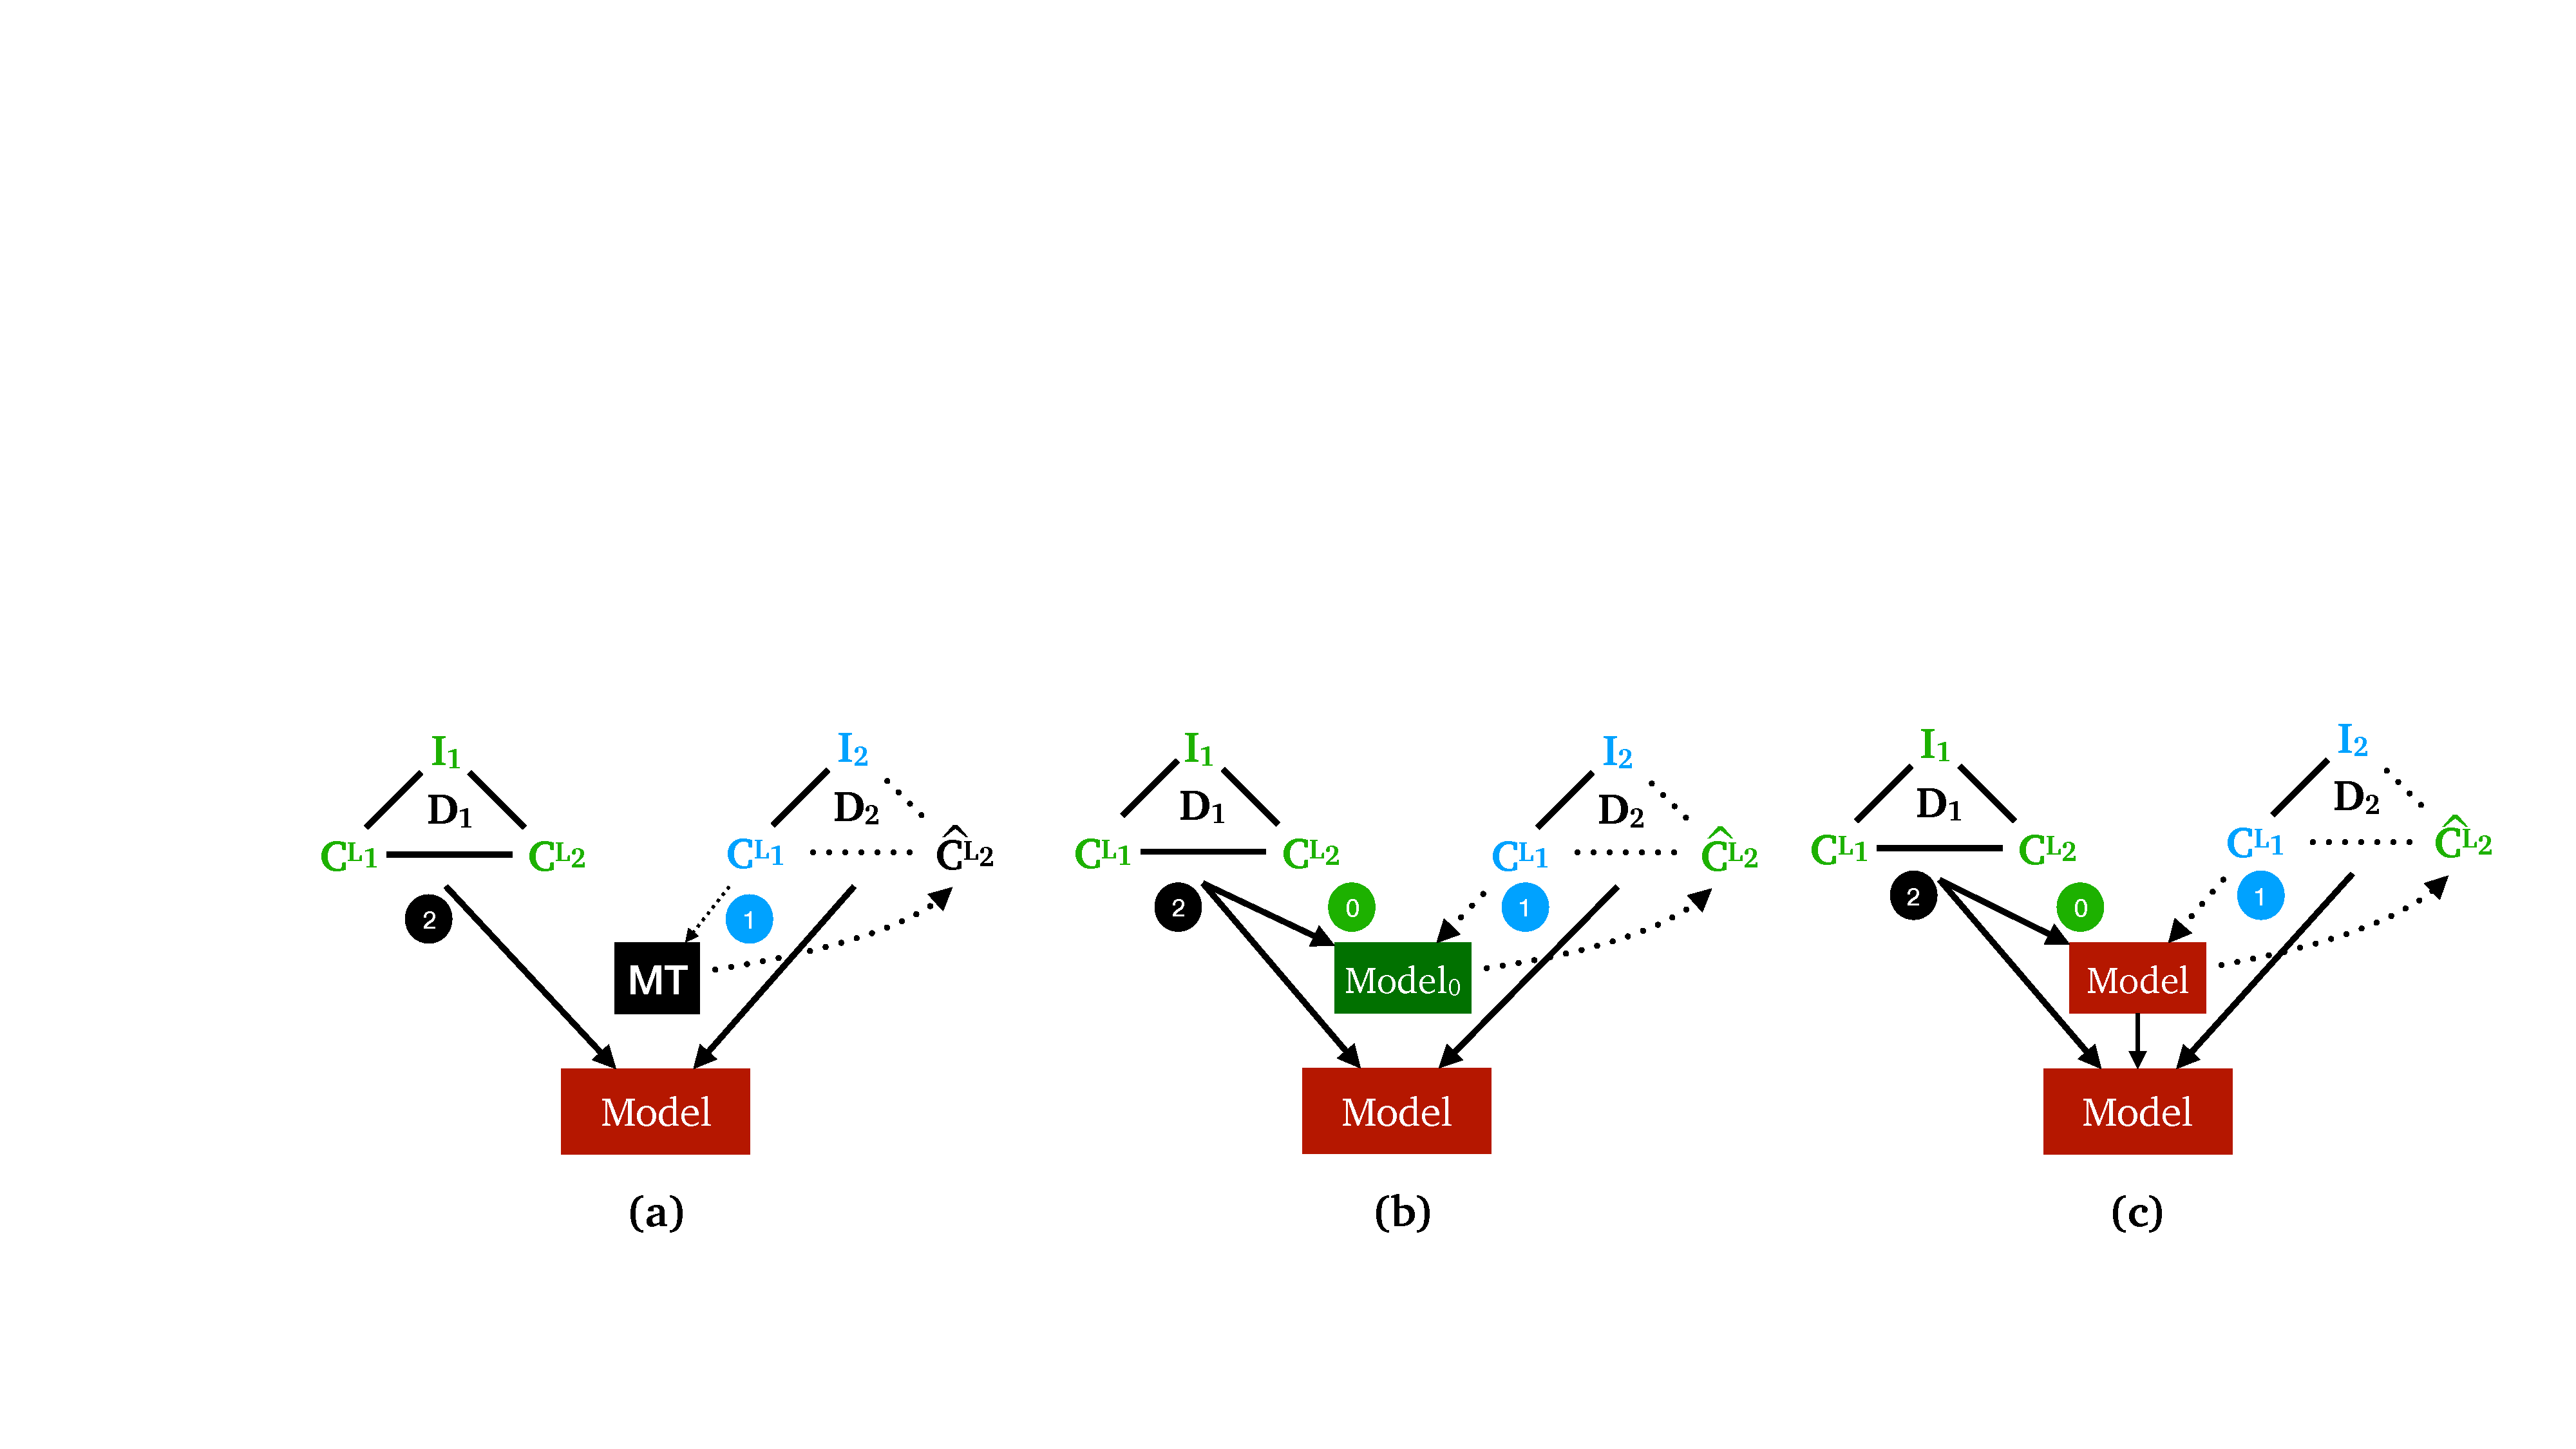
\includegraphics[width=1\textwidth]{assets/overview}
%  \caption{An overview of our approaches to creating an aligned dataset $\mathcal{D}_2$ of images ($\mathcal{I}$) with captions in two languages $\mathcal{C}^{\ell_1}$ and $\mathcal{C}^{\ell_2}$, from a $\mathcal{D}_2$ that only consists of $\mathcal{I}$-$\mathcal{C}^{\ell_2}$ pairs. In (a), we use an off-the-shelf machine translation system to create the $\hat{\mathcal{L}_2}$ data. The $\mathcal{D}_1$ and now-completed $\mathcal{D}_2$ data is used to train an image--sentence ranking model. In (b), we first train an ranking model on the $\mathcal{D}_1$ data, then we use the resulting Model$_0$ to transfer $\hat{\mathcal{L}_2}$ annotations given the $\mathcal{L}_1$ data to create pseudopairs. The resulting $\mathcal{D}_1$ and now-completed $\mathcal{D}_2$ data is used to train the final image--sentence ranking model. In (c), we follow the same process as (b), except that the initial model is fine-tuned with the pseudopairs.}\label{fig:overview}
%\end{figure*}

We adopt the model architecture and training procedure
of \cite{kadar2018conll} for the task of matching images with sentences. This task is defined as learning to rank the sentences associated with an image higher than other sentences in the data set, and vice-versa \citep{hodosh2013framing}. The model is comprised of 
a recurrent neural network language model and a 
convolutional neural network image encoder. 
The parameters of the 
language encoder are randomly initialized, while
the image encoder is pre-trained, frozen during 
training and followed by a linear layer which is
tuned for the task.  
The model is trained to make true pairs $<a,b>$ 
similar to each other, and contrastive pairs
$<\hat{a},b>$ and 
$<a,\hat{b}>$ dissimilar from each other in a joint
embedding space by minimizing the max-violation loss function
\citep{faghri2017vse++}:
%
\begin{equation}
\label{eq:maxviol}
\begin{split}
\mathcal{J}(a, b) = &\max_{<\hat{a}, b>}[\text{max}(0, \alpha - \text{s}(a,b) + \text{s}(\hat{a}, b))] \;+ \\ &\max_{<a, \hat{b}>}[\text{max}(0, \alpha - \text{s}(a,b) + \text{s}(a, \hat{b}))]
\end{split}
\end{equation}

In our experiments, the $<a, b>$ pairs are either image-caption pairs 
$<i, c>$ or caption--caption pairs $<c_a, c_b>$ (following \cite{gella2017image,kadar2018conll}).
When we train on $<i, c>$ pairs, we sample a batch
from an image--caption data set with uniform probability, encode the images and the sentences, and perform an update of the model parameters.
For the caption--caption objective, 
we follow \cite{kadar2018conll} and 
generate a sentence pair data set
by taking all pairs of sentences 
that belong to the same image
and are written in different languages: 5 English
and 5 German captions result in 25 English-German 
pairs. 
The sentences are encoded and we perform an update of 
the model parameters using the same loss. 
When training with both the image--caption and 
caption--caption (c2c) ranking tasks, 
we randomly select the task to perform with 
probability $p$=0.5. 

\subsection{Generating Synthetic Pairs}\label{sec:method:synthetic}

We propose two approaches to creating synthetic image--caption pairs to improve image--sentence ranking models when training with disjoint data sets. We assume the existence of datasets 
$\mathcal{D}_1$: $<\mathcal{I}^1$, $\mathcal{C}^{\ell_1}>$ and
$\mathcal{D}_2$: $<\mathcal{I}^2$, $\mathcal{C}^{\ell_2}>$
consisting of image--caption pairs $<i^1_i, c^{\ell_1}_i>$ and 
$<i^2_i, c^{\ell_2}_i>$ in 
languages $\ell_1$ and $\ell_2$, where the image sets do not overlap 
$\mathcal{I}^1 \cap \mathcal{I}^2 = \varnothing$. 
We seek to extend $<\mathcal{I}^2$, $\mathcal{C}^{\ell_2}>$ 
to a bilingual dataset with synthetic captions
$\hat{c}^{\ell_1}_i \in \hat{\mathcal{C}}^{\ell_1}$ 
in language $\ell_1$, resulting in a triplet data set 
$<\mathcal{I}^2$, $\hat{\mathcal{C}}^{\ell_1}$, $\mathcal{C}^{\ell_2}>$ 
consisting of triplets
 $<i^2_i, \hat{c}^{\ell_1}_i, c^{\ell_2}_i>$.
 We hypothesize that the new dataset will improve model performance because it will be trained to map the images to captions in both languages.%, \todo{because training with overlapping images is easier.}
 
 %we can train with the image--sentence and caption--caption ranking objectives \cite{D17-1303,kadar2018conll}.
%Figure \ref{fig:overview} presents an overview of our approaches to creating $\mathcal{I}$-$\mathcal{C}^\hat{\ell_1}$ pairs.

\subsection{Pseudopairs approach}\label{sec:method:pseudo}

\begin{comment}
Given two corpora $\mathcal{D}_1$ and $\mathcal{D}_2$, where $\mathcal{D}_1$ contains $<i_1, c_1>$ and $<i_2, c_2>$ pairs, and $\mathcal{D}_2$ contains $<i_2, c_1>$ pairs, we generate a \emph{pseudo-pair} corpora with noisy image-sentence pairs extracted from $D_1$. %Figure \ref{fig:overview} (b) shows an overview of this process.
In this paper, we create pseudo-pairs
in one direction $\mathcal{D}_1 \rightarrow \mathcal{D}_2$ leading 
to new image--caption pairs $<i_2, \hat{c}_2>$ for $\mathcal{D}_2$. 
We generate these pseudo-pairs using the cosine similarity between
sentence embeddings using a model trained on the $\mathcal{D}_1$ data. 
When generating 
pseudo-pairs $\mathcal{D}_1 \rightarrow \mathcal{D}_2$, we encode all 
captions $c_1 \in \mathcal{D}_2$ using the model trained on $\mathcal{D}_1$, and transfer the most similar $\hat{c}_2$ caption 
from $\mathcal{D}_1$ as its pair. This leads to $<c_2, c_1>$ pairs, and as a consequence to $<i_2, \hat{c}_2>$ pairs, and ultimately in a $\mathcal{D}_2$ corpus that contains $<i_1, c_1>$ and $<i_2, \hat{c_2}>$ pairs.
\end{comment}

Given two image-caption corpora  $<\mathcal{I}^1$, $\mathcal{C}^{\ell_1}>$  and  $<\mathcal{I}^2$, $\mathcal{C}^{\ell_2}>$ with pairs 
$<i^1_i, c^{\ell_1}_i>$ and $<i^2_i, c^{\ell_2}_i>$, we generate a \emph{pseudopair} corpus labeling each image in $\mathcal{I}^2$ with 
a caption from $\mathcal{C}^{\ell_1}$.
%Figure \ref{fig:overview} (b) shows an overview of this process.
In our experiments, we create pseudopairs
only in one direction  leading 
to new image--caption pairs $<i^2, \hat{c}^{\ell_1}>$. 

The pseudopairs are generated using the sentence representations of
the model trained on both corpora  $<\mathcal{I}^1$, $\mathcal{C}^{\ell_1}>$
and $<\mathcal{I}^2$, $\mathcal{C}^{\ell_2}>$ jointly. 
We encode all 
captions $c^{\ell_1}_i \in \mathcal{C}^{\ell_1}$ and 
 $c^{\ell_2}_i \in \mathcal{C}^{\ell_2}$ and for each $c^{\ell_2}_i$
find the most similar caption $\hat{c}^{\ell_1}_i$ using the cosine similarity between the sentence representations.
This leads to pairs $<c^{\ell_2}_i, \hat{c}^{\ell_1}_i>$ 
and as a result to triplets $<i^2_i, c^{\ell_2}_i, \hat{c}^{\ell_1}_i>$ .



\begin{comment}


This is summarized in Algorithm~\ref{alg:sentsim}.

\begin{algorithm}
\begin{algorithmic}
\State $pseudo\_caps \Leftarrow [\;]$
\For{$c_2 \in D_2$} 
    \State $\hat{c_2}$ = arg max $sim(c_1, C_1)$
    \State $pseudo\_caps$.add($\hat{c_2}$)
\EndFor
\end{algorithmic}
\caption{Pseudo-pairs based on sentence-similarities.}
\label{alg:sentsim}
\end{algorithm}
\end{comment}

\begin{comment}

\paragraph{2. Image-similarities} are the second option we explored. 
This approach is the same as the sentence similarities just the other way 
around as in as shown in Algorithm~\ref{alg:imgsim}.
\begin{algorithm}
\begin{algorithmic}
\State $pseudo\_imgs \Leftarrow [\;]$
\For{$i_2 \in D_2$} 
    \State $\hat{i_1}$ = arg max $sim(i_2, I_1)$
    \State $pseudo\_imgs$.add($\hat{i_1}$)
\EndFor
\end{algorithmic}
\caption{Pseudo-pairs based on image-similarities.}
\label{alg:imgsim}
\end{algorithm}
\end{comment}

\paragraph{Filtering}

Optionally we filter 
the resulting pseudopair set $\mathcal{C}^{\ell_1}$, in an attempt to
avoid misleading samples with three filtering strategies:

\begin{enumerate}
    \item No filtering.
    \item Keep top: keep items with similarity scores in the 75\% percentile; keep top 25\% 
    \item Remove bottom: keep items with similarity scores in the 25\%; remove bottom 25\%
\end{enumerate}

\paragraph{Fine-tuning vs. restart}
After the pseudopairs are generated we consider two 
options: re-train the model from scratch with all previous 
data sets adding the generated pseudopairs or fine-tunening with
same data sets and the additional pseudopairs.


\subsection{Translation approach}\label{sec:method:mt}
Given a corpus  
$<\mathcal{I}^2$, $\mathcal{C}^{\ell_2}>$ with pairs 
$<i^2_i, c^{\ell_2}_i>$, we use a machine 
translation system 
to translate each caption $c^{\ell_2}_i$ to a language $\ell_1$ leading to new image--caption pairs 
$<i^2_i, \hat{c}^{\ell_1}_i>$\footnote{\cite{li2016adding} used a similar approach to create Chinese captions for images in the Flickr8K dataset, but they used the translations to train a Chinese image captioning model.}. 
Any off-the-shelf translation system could be used to create the translated captions, e.g. an online service, such as Google Translate, or a pre-trained translation model. Here, we use a pre-trained model as it facilitates reproduction. 
%Figure \ref{fig:overview} (a) presents an overview of this approach.

%OpenNMT English-German model \cite{2017opennmt}\footnote{\url{https://s3.amazonaws.com/opennmt-models/wmt-ende_l2-h1024-bpe32k_release.tar.gz}}. The advantage of using the pre-trained system is th


\begin{comment}

Given two corpora $D^{\ell_1}$ and $D^{\ell_2}$ in two languages $\ell_1$ and $\ell_2$
containing image-sentence pairs $<i^{\ell_1}, s^{\ell_1}>$ and  $<i^{\ell_2}, s^{\ell_2}>$,
we generate a new \emph{pseudo-pair} corpus with pseudo image-sentence pairs extracted from the original $D^{\ell_1}$, $D^{\ell_2}$ corpora. Our solution is based on the
intuition that similar images are likely to have similar descriptions or conversely, similar sentences belong to similar images. This can be 
implemented by computing pairwise similarities between the image representations in the
corpora and taking the most similar pairs as new data points in the training data. 
In other words, for each image $i^{\ell_1}$ in $D^{\ell_1}$, we calculate its similarity to 
all of the images in $D^{\ell_2}$, and create a new data point $<i^{\ell_1}, i^{\ell_2}>$. 
From this new data point, we can extrapolate a 4-tuple of the similar images and their 
captions: $<i^{\ell_1}, i^{\ell_2}, s^{\ell_1}, s^{\ell_2}>$. 
The outcome of this process is three new noisy corpora: (1) $<i^{\ell_1}, s^{\ell_2}>$: 
images from $D^{\ell_1}$ paired with captions from $D^{\ell_2}$. (2) 
$<i^{\ell_2}, s^{\ell_1}>$: images from $D^{\ell_2}$ paired with captions 
from $D^{\ell_1}$; and (3) $<s^{\ell_1}, s^{\ell_2}>$: captions from $D^{\ell_1}$ paired 
with captions from $D^{\ell_2}$. We also perform this process in the other direction using the
intuition that similar captions are likely to belong to the similar images. For each caption
we calculate the similarity to all other captions in the other languages and perform the aforementioned procedure from this direction too.

\end{comment}